%==============================================================================
% BACHELOR THESIS - SYSTEM IMPLEMENTATION CHAPTER
% UniRemote & UniRobot Wireless Controller
%==============================================================================

\chapter{System Implementation}
\label{chap:implementation}

This chapter describes the hardware and software implementation of the universal wireless remote controller (UniRemote) and its corresponding robot-side receiver (UniRobot). The system is designed to provide a flexible, wireless interface for controlling various types of robots via serial communication.

%------------------------------------------------------------------------------
\section{System Overview}
%------------------------------------------------------------------------------

The system consists of two main units:

\begin{itemize}
    \item \textbf{UniRemote}: The handheld controller unit with joystick input, push button, OLED display, and wireless transmitter.
    \item \textbf{UniRobot}: The robot-side receiver that receives wireless commands and forwards them to the controlled robot via USB serial.
\end{itemize}

Communication between the two units is achieved using RFM69HCW radio modules operating at 433 MHz. This frequency was chosen as it falls within the ISM (Industrial, Scientific, Medical) band and does not require licensing in most countries.

\begin{figure}[H]
    \centering
    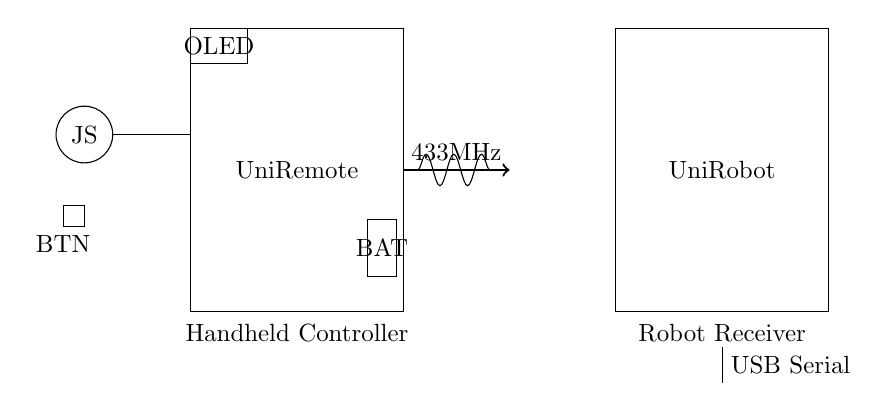
\begin{tikzpicture}[node distance=2cm, scale=0.9, transform shape]
        % Remote Unit
        \draw (0,0) rectangle (3,4) node[midway] {UniRemote};
        \node at (1.5, -0.3) {Handheld Controller};
        
        % Joystick
        \draw (-1.5, 2.5) circle (0.4) node {JS};
        \draw (-1.1, 2.5) -- (0, 2.5);
        
        % Button
        \draw (-1.5, 1.5) rectangle +(-0.3, -0.3) node[below] {BTN};
        
        % OLED
        \draw (0, 3.5) rectangle +(0.8, 0.5) node[midway] {OLED};
        
        % Battery
        \draw (2.5, 0.5) rectangle +(0.4, 0.8) node[midway] {BAT};
        
        % Radio waves
        \draw [->, thick] (3, 2) -- (4.5, 2) node[midway, above] {433MHz};
        \draw [decorate, decoration={snake, amplitude=2mm}] (3.2, 2) -- (4.3, 2);
        
        % Robot Unit
        \draw (6,0) rectangle (9,4) node[midway] {UniRobot};
        \node at (7.5, -0.3) {Robot Receiver};
        
        % USB output
        \draw (7.5, -0.5) -- (7.5, -1) node[midway, right] {USB Serial};
        
    \end{tikzpicture}
    \caption{System architecture overview}
    \label{fig:system_overview}
\end{figure}

%------------------------------------------------------------------------------
\section{Hardware Architecture}
%------------------------------------------------------------------------------

Both units are built around the Adafruit Feather M0 development board, which features the Atmel SAMD21 microcontroller with a 48 MHz ARM Cortex-M0+ core. The Feather form factor provides a compact solution with built-in USB support and battery charging capabilities.

\subsection{Hardware Components}

Table~\ref{tab:hardware_components} lists the key hardware components used in each unit.

\begin{table}[H]
    \centering
    \caption{Hardware components}
    \label{tab:hardware_components}
    \begin{tabular}{|l|l|l|}
        \hline
        \textbf{Component} & \textbf{UniRemote} & \textbf{UniRobot} \\
        \hline
        Microcontroller & Adafruit Feather M0 & Adafruit Feather M0 \\
        Wireless Module & RFM69HCW (433MHz) & RFM69HCW (433MHz) \\
        Display & SSD1306 OLED 128x32 & - \\
        Input & Analog Joystick & - \\
        Power & 3.7V LiPo Battery & USB Power \\
        \hline
    \end{tabular}
\end{table}

\subsection{Pin Configuration}

Tables~\ref{tab:remote_pins} and~\ref{tab:robot_pins} show the pin assignments for each unit.

\begin{table}[H]
    \centering
    \caption{UniRemote pin assignments}
    \label{tab:remote_pins}
    \begin{tabular}{|l|l|l|}
        \hline
        \textbf{Pin} & \textbf{Function} & \textbf{Connected To} \\
        \hline
        A4 & Analog Input & Joystick Y-axis \\
        A5 & Analog Input & Joystick X-axis \\
        A2 & Digital Input & Push Button \\
        A7 & Analog Input & Battery Voltage (via divider) \\
        5 & SPI CS & RFM69 Chip Select \\
        6 & Interrupt & RFM69 Interrupt \\
        10 & Digital Output & RFM69 Reset \\
        SDA & I2C Data & OLED Data \\
        SCL & I2C Clock & OLED Clock \\
        \hline
    \end{tabular}
\end{table}

\begin{table}[H]
    \centering
    \caption{UniRobot pin assignments}
    \label{tab:robot_pins}
    \begin{tabular}{|l|l|l|}
        \hline
        \textbf{Pin} & \textbf{Function} & \textbf{Connected To} \\
        \hline
        A5 & SPI CS & RFM69 Chip Select \\
        6 & Interrupt & RFM69 Interrupt \\
        A4 & Digital Output & RFM69 Reset \\
        \hline
    \end{tabular}
\end{table}

%------------------------------------------------------------------------------
\section{Software Architecture}
%------------------------------------------------------------------------------

The software is developed using the Arduino framework with PlatformIO as the build environment. The code is organized into modular components with separate files for each functional subsystem.

\subsection{Development Environment}

\begin{itemize}
    \item \textbf{Framework}: Arduino
    \item \textbf{Build System}: PlatformIO
    \item \textbf{Board}: Adafruit Feather M0 (SAMD21)
    \item \textbf{Communication Speed}: 115200 baud
\end{itemize}

The following libraries are used:
\begin{itemize}
    \item \texttt{RFM69} (LowPowerLab) - Radio communication
    \item \texttt{Adafruit SSD1306} - OLED display control
    \item \texttt{SPIFlash} - Optional external flash (available but unused)
\end{itemize}

%------------------------------------------------------------------------------
\subsection{UniRemote Software}
%------------------------------------------------------------------------------

The UniRemote firmware handles joystick reading, wireless transmission, and status display.

\subsubsubsection{Joystick Module}

The joystick provides two analog signals representing the X and Y positions. These are read using the microcontroller's 10-bit ADC and converted to 8-bit values by right-shifting by 2 bits:

\begin{lstlisting}[language=C++]
void readJoystick(uint8_t *x, uint8_t *y) {
    *x = analogRead(A5) >> 2;
    *y = analogRead(A4) >> 2;
}
\end{lstlisting}

The joystick axes are mapped as follows:
\begin{itemize}
    \item X-axis: Left (0) to Right (255)
    \item Y-axis: Up (0) to Down (255)
\end{itemize}

\subsubsubsection{Radio Module}

The RFM69HCW radio is initialized with the following parameters:
\begin{itemize}
    \item Frequency: 433 MHz
    \item Network ID: 42
    \item Node ID: 2 (UniRemote)
    \item Target Node ID: 1 (UniRobot)
\end{itemize}

The \texttt{sendData()} function transmits the joystick position and button state, then waits for an acknowledgment (ACK) that contains the robot-side RSSI and battery information:

\begin{lstlisting}[language=C++]
bool sendData(uint8_t x, uint8_t y, uint8_t button, 
              int16_t *masterRSSI, int8_t *slaveRSSI, uint8_t *battery) {
    uint8_t packet[3];
    packet[0] = x;
    packet[1] = y;
    packet[2] = button;

    if (!radio.sendWithRetry(TONODEID, packet, sizeof(packet), 5, 20)) {
        Serial.println("No ACK received");
        return false;
    }

    *masterRSSI = radio.RSSI;
    *slaveRSSI = (int8_t)radio.DATA[0];
    *battery = radio.DATA[1];

    return true;
}
\end{lstlisting}

The \texttt{sendWithRetry()} function attempts up to 5 transmissions with a 20ms timeout between attempts, providing reliable delivery.

\subsubsubsection{Display Module}

The SSD1306 OLED display shows real-time status information:
\begin{itemize}
    \item RSSI (Received Signal Strength Indicator)
    \item Remote battery voltage
    \item Robot battery voltage (from ACK)
\end{itemize}

\subsubsubsection{Main Loop}

The main loop executes at approximately 10 Hz (100ms delay):

\begin{enumerate}
    \item Read joystick X and Y positions
    \item Read remote battery voltage (via analog divider)
    \item Transmit data packet to UniRobot
    \item Update OLED display with received information
    \item Wait 100ms before next iteration
\end{enumerate}

%------------------------------------------------------------------------------
\subsection{UniRobot Software}
%------------------------------------------------------------------------------

The UniRobot firmware runs on the robot side and receives commands from the remote.

\subsubsubsection{Radio Initialization}

The receiver uses identical radio parameters but with different node IDs:
\begin{itemize}
    \item Frequency: 433 MHz
    \item Network ID: 42
    \item Node ID: 1 (UniRobot)
    \item Target Node ID: 2 (UniRemote)
\end{itemize}

\subsubsubsection{Data Reception}

The \texttt{transiver\_receive()} function continuously checks for incoming packets:

\begin{lstlisting}[language=C++]
void transiver_receive() {
    if (radio.receiveDone()) {
        if (radio.ACKRequested()) {
            uint8_t ackPayload[2];
            ackPayload[0] = (uint8_t)radio.RSSI;
            ackPayload[1] = BATTERY_PLACEHOLDER;
            radio.sendACK(ackPayload, sizeof(ackPayload));
        }

        uint8_t x = radio.DATA[0];
        uint8_t y = radio.DATA[1];
        uint8_t button = radio.DATA[2];

        handleDataPacket(x, y, button);
    }
}
\end{lstlisting}

When a packet is received, an ACK is sent back containing the RSSI reading and a placeholder battery value. The received data (X, Y, button) is passed to \texttt{handleDataPacket()} for processing.

\subsubsubsection{Data Handling}

Currently, the received data is printed to the serial monitor:

\begin{lstlisting}[language=C++]
void handleDataPacket(uint8_t x, uint8_t y, uint8_t button) {
    static int16_t lastRSSI = 0;
    lastRSSI = radio.RSSI;

    Serial.print("x:"); Serial.print(x);
    Serial.print(", y:"); Serial.print(y);
    Serial.print(", btn:"); Serial.print(button);
    Serial.print(", rssi:"); Serial.println(lastRSSI);
}
\end{lstlisting}

This serial output can be consumed by any robot that accepts serial commands via USB.

%------------------------------------------------------------------------------
\section{Communication Protocol}
%------------------------------------------------------------------------------

The communication protocol is designed for reliability while maintaining low latency.

\subsection{Packet Structure}

\begin{table}[H]
    \centering
    \caption{Transmitted packet structure (Remote $\rightarrow$ Robot)}
    \label{tab:packet_tx}
    \begin{tabular}{|c|c|c|}
        \hline
        \textbf{Byte 0} & \textbf{Byte 1} & \textbf{Byte 2} \\
        \hline
        X Position & Y Position & Button State \\
        (uint8) & (uint8) & (uint8) \\
        \hline
    \end{tabular}
\end{table}

\begin{table}[H]
    \centering
    \caption{ACK packet structure (Robot $\rightarrow$ Remote)}
    \label{tab:packet_ack}
    \begin{tabular}{|c|c|c|}
        \hline
        \textbf{Byte 0} & \textbf{Byte 1} \\
        \hline
        RSSI & Battery Level \\
        (int8) & (uint8) \\
        \hline
    \end{tabular}
\end{table}

\subsection{Reliability Features}

\begin{itemize}
    \item \textbf{Automatic Retransmission}: Up to 5 retry attempts with 20ms delays
    \item \textbf{ACK Mechanism}: Confirmed delivery with RSSI feedback
    \item \textbf{Error Detection}: Built into RFM69 hardware
\end{itemize}

%------------------------------------------------------------------------------
\section{Current Limitations and Future Work}
%------------------------------------------------------------------------------

The current implementation provides the foundation for a universal remote controller but has several areas for enhancement:

\begin{enumerate}
    \item \textbf{Serial Protocol}: A standardized command protocol for robots needs to be defined to ensure compatibility across different robot types.
    
    \item \textbf{Robot Control}: The UniRobot currently only outputs serial data; actual motor control logic needs to be implemented.
    
    \item \textbf{Battery Monitoring}: The robot-side battery reading uses a placeholder value (100) and should be replaced with actual voltage measurement.
    
    \item \textbf{Control Modes}: Different control schemes (tank steering, arcade-style, RC mode) would increase versatility.
    
    \item \textbf{Address Expansion}: Network addressing could support multiple remotes and robots simultaneously.
    
    \item \textbf{Encryption}: Optional encryption could be added for secure operation.
\end{enumerate}

%------------------------------------------------------------------------------
\section{Summary}
%------------------------------------------------------------------------------

This chapter presented the implementation of a wireless universal remote controller system. The UniRemote unit reads joystick input and transmits commands via RFM69HCW radio modules at 433 MHz. The UniRobot receiver outputs the received commands via USB serial, allowing any robot with serial input capability to be controlled.

The modular design allows the remote to be adapted for different robot types by modifying the robot-side code while keeping the remote hardware unchanged. The current implementation provides reliable wireless communication with acknowledgment feedback, forming a solid foundation for further development.

%==============================================================================
% END OF CHAPTER
%==============================================================================